% Options for packages loaded elsewhere
\PassOptionsToPackage{unicode}{hyperref}
\PassOptionsToPackage{hyphens}{url}
\PassOptionsToPackage{dvipsnames,svgnames,x11names}{xcolor}
%
\documentclass[
  12pt]{article}

\usepackage{amsmath,amssymb}
\usepackage{iftex}
\ifPDFTeX
  \usepackage[T1]{fontenc}
  \usepackage[utf8]{inputenc}
  \usepackage{textcomp} % provide euro and other symbols
\else % if luatex or xetex
  \usepackage{unicode-math}
  \defaultfontfeatures{Scale=MatchLowercase}
  \defaultfontfeatures[\rmfamily]{Ligatures=TeX,Scale=1}
\fi
\usepackage{lmodern}
\ifPDFTeX\else  
    % xetex/luatex font selection
\fi
% Use upquote if available, for straight quotes in verbatim environments
\IfFileExists{upquote.sty}{\usepackage{upquote}}{}
\IfFileExists{microtype.sty}{% use microtype if available
  \usepackage[]{microtype}
  \UseMicrotypeSet[protrusion]{basicmath} % disable protrusion for tt fonts
}{}
\makeatletter
\@ifundefined{KOMAClassName}{% if non-KOMA class
  \IfFileExists{parskip.sty}{%
    \usepackage{parskip}
  }{% else
    \setlength{\parindent}{0pt}
    \setlength{\parskip}{6pt plus 2pt minus 1pt}}
}{% if KOMA class
  \KOMAoptions{parskip=half}}
\makeatother
\usepackage{xcolor}
\setlength{\emergencystretch}{3em} % prevent overfull lines
\setcounter{secnumdepth}{5}
% Make \paragraph and \subparagraph free-standing
\ifx\paragraph\undefined\else
  \let\oldparagraph\paragraph
  \renewcommand{\paragraph}[1]{\oldparagraph{#1}\mbox{}}
\fi
\ifx\subparagraph\undefined\else
  \let\oldsubparagraph\subparagraph
  \renewcommand{\subparagraph}[1]{\oldsubparagraph{#1}\mbox{}}
\fi


\providecommand{\tightlist}{%
  \setlength{\itemsep}{0pt}\setlength{\parskip}{0pt}}\usepackage{longtable,booktabs,array}
\usepackage{calc} % for calculating minipage widths
% Correct order of tables after \paragraph or \subparagraph
\usepackage{etoolbox}
\makeatletter
\patchcmd\longtable{\par}{\if@noskipsec\mbox{}\fi\par}{}{}
\makeatother
% Allow footnotes in longtable head/foot
\IfFileExists{footnotehyper.sty}{\usepackage{footnotehyper}}{\usepackage{footnote}}
\makesavenoteenv{longtable}
\usepackage{graphicx}
\makeatletter
\def\maxwidth{\ifdim\Gin@nat@width>\linewidth\linewidth\else\Gin@nat@width\fi}
\def\maxheight{\ifdim\Gin@nat@height>\textheight\textheight\else\Gin@nat@height\fi}
\makeatother
% Scale images if necessary, so that they will not overflow the page
% margins by default, and it is still possible to overwrite the defaults
% using explicit options in \includegraphics[width, height, ...]{}
\setkeys{Gin}{width=\maxwidth,height=\maxheight,keepaspectratio}
% Set default figure placement to htbp
\makeatletter
\def\fps@figure{htbp}
\makeatother

\addtolength{\oddsidemargin}{-.5in}%
\addtolength{\evensidemargin}{-1in}%
\addtolength{\textwidth}{1in}%
\addtolength{\textheight}{1.7in}%
\addtolength{\topmargin}{-1in}%

\usepackage{amsthm}
\newtheorem{ass}{Assumption}
% \usepackage{mathtools}
\usepackage[final, nomargin, inline, nomarginclue, author=HM]{fixme}
% \fxusetargetlayout{color}
\fxsetface{inline}{\color{blue}}
\fxsetface{env}{\color{blue}}
% \usepackage{amsmath}
% \usepackage[final,nomargin,index,inline, author=]{fixme}
% \usepackage{bbm}
\usepackage{unicode-math}
\usepackage{tabularx}
\usepackage{adjustbox}
% \usepackage{amsmath}
% - \usepackage{longtable}
% - \usepackage{booktabs}
% - \usepackage{graphicx}
% \newtheorem{definition}{Definition}
% \newtheorem{theo}{Theorem}
% \newtheorem{lemma}{Lemma}
% \newtheorem{ass}{Assumption}
% \usepackage{xkvltxp}
% -  #final or draft
% - \fxsetup{envlayout=color, targetlayout=color}
% - \fxsetface{inline}{\color{blue}}

% kableExtra required packages:
\usepackage{booktabs}
\usepackage{longtable}
% \usepackage{array}
% \usepackage{multirow}
% \usepackage{wrapfig}
% \usepackage{float}
% \usepackage{colortbl}
% \usepackage{pdflscape}
% \usepackage{tabu}
\usepackage{threeparttable}
\usepackage{threeparttablex}
% \usepackage[normalem]{ulem}
% \usepackage{makecell}
% \usepackage{xcolor}
\usepackage{booktabs}
\usepackage{longtable}
\usepackage{array}
\usepackage{multirow}
\usepackage{wrapfig}
\usepackage{float}
\usepackage{colortbl}
\usepackage{pdflscape}
\usepackage{tabu}
\usepackage{threeparttable}
\usepackage{threeparttablex}
\usepackage[normalem]{ulem}
\usepackage{makecell}
\usepackage{xcolor}
\makeatletter
\makeatother
\makeatletter
\makeatother
\makeatletter
\@ifpackageloaded{caption}{}{\usepackage{caption}}
\AtBeginDocument{%
\ifdefined\contentsname
  \renewcommand*\contentsname{Table of contents}
\else
  \newcommand\contentsname{Table of contents}
\fi
\ifdefined\listfigurename
  \renewcommand*\listfigurename{List of Figures}
\else
  \newcommand\listfigurename{List of Figures}
\fi
\ifdefined\listtablename
  \renewcommand*\listtablename{List of Tables}
\else
  \newcommand\listtablename{List of Tables}
\fi
\ifdefined\figurename
  \renewcommand*\figurename{Figure}
\else
  \newcommand\figurename{Figure}
\fi
\ifdefined\tablename
  \renewcommand*\tablename{Table}
\else
  \newcommand\tablename{Table}
\fi
}
\@ifpackageloaded{float}{}{\usepackage{float}}
\floatstyle{ruled}
\@ifundefined{c@chapter}{\newfloat{codelisting}{h}{lop}}{\newfloat{codelisting}{h}{lop}[chapter]}
\floatname{codelisting}{Listing}
\newcommand*\listoflistings{\listof{codelisting}{List of Listings}}
\makeatother
\makeatletter
\@ifpackageloaded{caption}{}{\usepackage{caption}}
\@ifpackageloaded{subcaption}{}{\usepackage{subcaption}}
\makeatother
\makeatletter
\@ifpackageloaded{tcolorbox}{}{\usepackage[skins,breakable]{tcolorbox}}
\makeatother
\makeatletter
\@ifundefined{shadecolor}{\definecolor{shadecolor}{rgb}{.97, .97, .97}}
\makeatother
\makeatletter
\makeatother
\makeatletter
\makeatother
\ifLuaTeX
  \usepackage{selnolig}  % disable illegal ligatures
\fi
\usepackage[]{natbib}
\bibliographystyle{agsm}
\IfFileExists{bookmark.sty}{\usepackage{bookmark}}{\usepackage{hyperref}}
\IfFileExists{xurl.sty}{\usepackage{xurl}}{} % add URL line breaks if available
\urlstyle{same} % disable monospaced font for URLs
\hypersetup{
  pdftitle={Tax evasion and productivity},
  pdfauthor={Hans Martinez},
  pdfkeywords={Tax Evasion, Cost Overreporting, Production Function
Estimation, Productivity},
  colorlinks=true,
  linkcolor={blue},
  filecolor={Maroon},
  citecolor={Blue},
  urlcolor={Blue},
  pdfcreator={LaTeX via pandoc}}


\begin{document}


\def\spacingset#1{\renewcommand{\baselinestretch}%
{#1}\small\normalsize} \spacingset{1}


%%%%%%%%%%%%%%%%%%%%%%%%%%%%%%%%%%%%%%%%%%%%%%%%%%%%%%%%%%%%%%%%%%%%%%%%%%%%%%

\date{November 3, 2023}
\title{\bf Tax evasion and productivity}
\author{
Hans Martinez\thanks{email: hmarti33@uwo.ca. I thank my supervisors
Salvador Navarro, David Rivers, and Victor Aguiar for their guidance.}\\
Department of Economics, University of Western Ontario\\
}
\maketitle

\bigskip
\bigskip
\begin{abstract}
Corporate tax evasion through cost overreporting spreads internationally
causing governments significant tax revenue losses. Detecting and
measuring the magnitude of tax evasion remains a challenge, even for the
few studies on overreporting where researchers can exploit
administrative data. Moreover, if this evasion strategy accounts for
economic losses as large as reported, then cost overreporting might bias
estimates of production functions, especially productivity. This paper
addresses both issues. I first provide a novel strategy to estimate cost
overreporting using commonly available firm-level data. I then formally
show that ignoring cost overreporting leads to downward biased
productivity estimates. Finally, I demonstrate how to recover
productivity in the presence of tax evasion.
\end{abstract}

\noindent%
{\it Keywords:} Tax Evasion, Cost Overreporting, Production Function
Estimation, Productivity
\vfill

\newpage
\spacingset{1.9} % DON'T change the spacing!
\ifdefined\Shaded\renewenvironment{Shaded}{\begin{tcolorbox}[interior hidden, breakable, enhanced, borderline west={3pt}{0pt}{shadecolor}, sharp corners, frame hidden, boxrule=0pt]}{\end{tcolorbox}}\fi

\hypertarget{updates}{%
\section*{Updates}\label{updates}}
\addcontentsline{toc}{section}{Updates}

\begin{itemize}
\tightlist
\item
  Simple model that incorporates evasion decision and size endogenously
\item
  Colombian Corporate tax system
\item
  Identification strategy for Colombia
\end{itemize}

\hypertarget{a-parsimonious-model-of-tax-evasion-through-input-overreporting}{%
\section{A parsimonious model of tax evasion through input
overreporting}\label{a-parsimonious-model-of-tax-evasion-through-input-overreporting}}

Price-taking firms maximize expected after-tax profits. Firms choose the
flexible input \(M_{it}\) to produce output \(Y_{it}\) given output and
input prices \(\{P_{t}, \rho_t\}\), a common technology, the production
function (Equation~\ref{eq-prod-fn}), and their productivity
\(\omega_{it}\).

\begin{equation}\protect\hypertarget{eq-prod-fn}{}{
Y_{it}=G(M_{it})\exp(\omega_{it}+\varepsilon_{it})
}\label{eq-prod-fn}\end{equation}

As standard in the literature, productivity \(\omega_{it}\) is known to
firms when they take input decisions. This is the well-known endogeneity
problem of simultaneity. On the other hand, firms face output shocks.
The output shock \(\varepsilon_{it}\) is not part of the firms'
information set.

The model departs from the literature by allowing firms to overreport
their inputs \(e_{it}\) to reduce their tax burden and optimize
after-tax profits. Firms, then, consider in their optimization problem
the profit tax \(\tau\), the evasion penalty/cost \(\kappa(e)\), and the
probability of detection \(q_{it}(e_{it}|\theta_{it})\).

Firms solve Equation~\ref{eq-eva}
\begin{equation}\protect\hypertarget{eq-eva}{}{
\begin{aligned}
  \max_{M_{it}, e_{it}\in [0,\infty), } [1-q_{it}(e_{it}|\theta_{it})]&\left[(P_t\mathbb{E}[Y_{it}]-\rho_{t} M_{it})-\tau\left(P_t\mathbb{E}[Y_{it}]-\rho_{t} (M_{it}+e_{it})\right)\right]\\
  +q_{it}(e_{it}|\theta_{it})&\left[(1-\tau)(P_t\mathbb{E}[Y_{it}]-\rho_{t} M_{it})-\kappa(e)\right] \\
  \text{s.t. }\; Y_{it}=G(M_{it})\exp(\omega_{it}+\varepsilon_{it})
\end{aligned}
}\label{eq-eva}\end{equation}

The probability of detection \(q_{it}(e_{it}|\theta_{it})\) is
monotonically increasing in the amount evaded \(e_{it}\), conditional on
the type of the firm \(\theta_{it}\). Intuitively, for a given type,
firms that evade more are more likely to get caught.

The type of the firm \(\theta_{it}\) might be discrete, like the type of
juridical organization, or continuous, like the level of
revenue\footnote{Level of revenue is a common measure for fiscal
  authorities to determine a firm's taxes and/or level of scrutiny,
  e.g., Mexico, Spain, Colombia, Ecuador, and Chile (?).}. Some types
might be more likely to be detected if the firm engages in tax evasion.
For example, in contrast to other types of juridical organizations in
Colombia, corporations are closely supervised and are required to have
an auditor. That is, for a given level of tax evasion \(e_0\) and two
different types \(\theta' \not= \theta \in \mathbfcal{\Theta}\), then
\(q(e_0|\theta')\ge q(e_0|\theta)\).

If the type \(\theta\) is continuous, it might be a function of inputs;
for example, level of revenue. Firms will then affect their probability
of detection \(q(e|\theta)\) in two ways: directly, by choosing how much
they evade \(e\); and indirectly, when choosing inputs \(M\).

The optimal decision of the firm will depend on the fiscal environment
\(\Gamma=\{\tau, \kappa, q \}\), namely the tax rates, the penalty/cost
of detection, and the probability of detection.

The firms' problem (Equation~\ref{eq-eva}) can be rewritten as follows,
\[
\begin{aligned}
  \max_{M_{it},e_{it}} \mathbb{E}[\pi_{it}|\Gamma] = &(1-\tau)\left(\mathbb{E}[Y_{it}]-\frac{\rho_{t}}{P_t} M_{it}\right)+[1-q_{it}(e_{it}|\theta_{it})]\left(\frac{\rho_{t}}{P_t}e_{it}\tau\right)
  -q_{it}(e_{it}|\theta_{it})\kappa(e_{it}) \\
  &\text{s.t. }\; Y_{it}=G(M_{it})\exp(\omega_{it}+\varepsilon_{it})
\end{aligned}
\]

Intuitively, if the firm overreports her inputs' cost, she will get the
share of the value she overreported with probability \((1-q)\) and she
will be penalized with probability \(q\).

Assuming well-behaved functions and no corner solutions, the first-order
conditions lead to the following system of differential equations,

\begin{equation}\protect\hypertarget{eq-foc-cont-m}{}{
G_M(M_{it})\exp(\omega_{it})\mathcal{E}-\frac{\rho_{t}}{P_t} = \frac{1}{(1-\tau)}\frac{\partial q(e_{it}|\theta_{it})}{\partial \theta_{it}}\frac{\partial \theta_{it}}{\partial M}\left[\frac{\rho_t}{P_t}e_{it}\tau+\kappa(e_{it})\right]
}\label{eq-foc-cont-m}\end{equation}

\begin{equation}\protect\hypertarget{eq-foc-cont-e}{}{
[1-q(e_{it}|\theta_{it})]\frac{\rho_t}{P_t}\tau-q(e_{it}|\theta_{it})\kappa'(e_{it})=q'(e_{it}|\theta_{it})\left[\frac{\rho_t}{P_t}\tau e_{it} + \kappa(e_{it})\right]
}\label{eq-foc-cont-e}\end{equation}

where \(\mathbfcal{E}=\mathbb{E}[\exp(\varepsilon_{it})]\). The type of
firms is continuous and increasing on the input. The probability of
detection is increasing in the type continuum. In particular,
\(\frac{\partial q(e_{it}|\theta_{it})}{\partial \theta_{it}}\frac{\partial \theta_{it}}{\partial M}\ge0\).

The left-hand side of Equation~\ref{eq-foc-cont-m} is the familiar
marginal output of inputs and the price ratio. In the absence of
incentives' distortions induced by the fiscal environment, they are
equal. But now, the equality holds no more. There's a wedge arising from
the fiscal environment. The right-hand side of the equation is positive
by the assumptions of the model.

Equation~\ref{eq-foc-cont-e} solves for the optimal evasion decision.
The left-hand side is the marginal benefit net of the marginal cost of
evasion. The right-hand side is the rate of change of the probability of
detection due to a change in evasion weighted by the benefit and cost of
evading.

\hypertarget{case-1-independece-qethetaqe-and-kappaekappa_0}{%
\subsection{\texorpdfstring{Case 1 (Independece): \(q(e|\theta)=q(e)\)
and
\(\kappa(e)=\kappa_0\)}{Case 1 (Independece): q(e\textbar\textbackslash theta)=q(e) and \textbackslash kappa(e)=\textbackslash kappa\_0}}\label{case-1-independece-qethetaqe-and-kappaekappa_0}}

Consider the case when the probability of detection is independent of
type, \(q(e|\theta)=q(e)\), and the evasion cost is constant
\(\kappa(e)=\kappa_0\). This could be the case if the type is the
juridical organization of the firm and the penalty of evading is
constant for the type of juridical organization. The type of the firm,
and therefore the probability of detection, does not change with the
firm's input decisions.

In this case, the first-order conditions of Equation~\ref{eq-eva} with
respect to the input \(M_{it}\) and the tax evasion \(e_{it}\) yield the
following

\begin{equation}\protect\hypertarget{eq-foc:ind}{}{
G_M(M_{it})\exp(\omega_{it})\mathcal{E}=\frac{\rho_{t}}{P_t}
}\label{eq-foc:ind}\end{equation}

\begin{equation}\protect\hypertarget{eq-foc:eva:ind}{}{
e_{it}=\frac{1-q(e_{it})}{q'(e_{it})}-\frac{\kappa_0}{\frac{\rho_{t}}{P_t}\tau}
}\label{eq-foc:eva:ind}\end{equation}

Equation~\ref{eq-foc:ind}, the well-known optimality condition, says
that the price ratio is equal to the marginal product of the inputs.

Likewise, Equation~\ref{eq-foc:eva:ind} reveals the firms' optimal tax
evasion decision decreases if the probability of detection \(q(e_{it})\)
or the penalty of evading \(\kappa\) increases. Tax evasion also depends
on how sensitive the probability of detection is to the level of evasion
\(q'(e)\). In particular, greater sensibility will result in lower
levels of evasion.

Note that the net change of tax evasion due to an increase in the
relative prices \(\frac{\rho_{t}}{P_t}\) or the tax rate \(\tau\) is not
evident at first sight. The net effect will also depend on the change in
the detection probability induced by the changes in the relative prices
or the tax rate. In particular, an increase in relative prices
\(\frac{\rho_{t}}{P_t}\) or the tax rate \(\tau\) will incentivize a
higher tax evasion level, however, a higher tax evasion level will
increase the probability of detection ---depending on the shape of the
probability as a function of \(e\)---, so it will deter higher levels of
evasion. An increase in the tax rate, for instance, will only increase
tax evasion if the change in the tax rates increases the incentives to
evade more than the decrease in the incentives due to the changes in the
detection probability.

Formally, suppose a firm increases its tax evasion, \(e_1-e_0>0\)
because of an increase in taxes \(\tau_1>\tau_0\). Then, it follows that

\[
\left(\frac{\tau_1-\tau_0}{\tau_1\tau_0}\right)\frac{P\kappa}{\rho}>
  \left(\frac{1-q(e_1)}{q'(e_1)}-\frac{1-q(e_0)}{q'(e_0)}\right)
\]

The change in the probability of detection weighted by the slope of the
probability function should be less than the change in the tax rate
weighted by the penalty of evading and the relative prices\footnote{An
  analogous condition for an increase in relative prices leading to
  higher levels of tax evasion exists. Under this condition, the model
  is consistent with the literature that macroeconomic downturns lead to
  higher evasion.}.

\hypertarget{case-2-spain-discrete-increase-in-the-probability-of-detection-after-a-certain-threshold-of-revenue}{%
\subsection{Case 2 (Spain): Discrete increase in the probability of
detection after a certain threshold of
revenue}\label{case-2-spain-discrete-increase-in-the-probability-of-detection-after-a-certain-threshold-of-revenue}}

In Spain, the Large Taxpayers Unit (LTU) of the tax authority focuses
exclusively on firms with total operating revenue above 6 million euros.
The LTU has more auditors per taxpayer than the rest of the tax
authority, and these auditors are on average more experienced and better
trained to deal with the most complex taxpayers. This LTU creates a
discontinuity in the monitoring effort of the tax authority.
Consequently, at this arbitrary revenue level, the probability of
detection increases discretely \citep{Almunia2018}.

In this scenario, depending on the productivity shock, the firm might be
better off choosing not to produce past the revenue threshold. Indeed,
for a relevant range of productivity draws
\(\Omega^B=[\omega^L, \omega^H]\), the firms will not choose to grow
past the revenue threshold if the expected after-tax profits of staying
small are greater than the expected after-tax profits of growing.

In the model, there is now a threshold of revenue \(\theta^L\) after
which the probability of detection increases discretely. To make things
simpler, assume that before the threshold, the probability changes as a
function of evasion but does not vary conditional on size. After the
threshold, the probability increases for every level of evasion but does
not vary conditional on size.

Formally, let \(\Theta_{L} = \{\theta_i : \theta_{i} < \theta^L \}\) and
\(\Theta_{H} = \{\theta_i : \theta_{i} \ge \theta^L \}\), then for all
\(e_0\) and \(\theta'_i\not=\theta_i\),
\(q(e_0|\theta_i \in \Theta_k)=q(e_0|\theta'_i \in \Theta_k)\) with
\(k=\{L,H\}\), but
\(q(e_0|\theta'_i \in \Theta_H)\ge q(e_0|\theta_i \in \Theta_L)\).

Firms' revenue with productivity draw \(\omega^L\) corresponds exactly
to the enforcement threshold \(\theta^L\). Production and reporting
decisions of firms with productivity draws below \(\omega^L\) are not
affected by the change in the probability of detection. Firms choose
their inputs according to Equation~\ref{eq-foc:ind} and their evasion
decision according to Equation~\ref{eq-foc-cont-e}. Firms with
productivity draws above \(\omega^U\)

Firms with productivity \(\omega_{i}\in \Omega^B\) will choose the input
level \(\tilde{M}_{i}\) resulting in an expected revenue below the
threshold \(\theta_{i}<\theta^L\), if the expected after-tax profit of
staying small are greater than growing,
\(\mathbb{E}[\pi_{i}|\Theta_L, \Omega^B]-\mathbb{E}[\pi_{i}|\Theta_H, \Omega^B]\ge0\).

The optimal input choice \(M^*_{i}\) for firms with productivity
\(\omega_i\in\Omega^B\) implies an expected revenue greater than or
equal to the threshold \(\theta^*_{i}\ge \theta^L\). Let the expected
profits given \(M^*_{i}\) and the optimal tax evasion in the range of
size \(\theta_l\), \(e^*_{it}\), is
\(\pi_l\equiv\mathbb{E}[\pi(M^*_{it}, e^*_{it})|\theta_l]\). Let
\(\tilde{M}_{it}\) be the input level such that the expected revenue is
below the threshold \(\tilde{s}_{it}<\theta^L\) and \(\tilde{e}_{it}\)
be the optimal tax evasion in the range of size \(\theta_s\). Let also
the expected profits of staying small are
\(\pi_s\equiv\mathbb{E}[\pi(\tilde{M}_{it},\tilde{e}_{it})|\theta_s]\).

In this second case, therefore, firms might optimally choose to remain
small if, for a low productivity shock, the expected profits of not
growing are greater than the expected profits of growing
\(\pi_l<\pi_s\). Firms choosing to remain small will lead to a bunching
below the threshold in the size distribution of firms.

Besides the higher levels of evasion before the threshold ---simply
because of the higher probability of detection---, we can also expect
bunching firms to evade more than their similar-sized peers. At
\(\tilde{M}_{it}\), the optimization condition of
Equation~\ref{eq-foc:ind} no longer holds, hence, the marginal product
of the input is now greater than the relative prices. Therefore,
according to Equation~\ref{eq-foc:eva:ind}, bunching firms would
compensate for their \emph{higher} costs by increasing overreporting.

\hypertarget{whats-new}{%
\subsubsection{What's new?}\label{whats-new}}

\begin{itemize}
\tightlist
\item
  GOPF framework with public data vs bunching estimator with private
  administrative data
\item
  Focus on input overreporting rather than on revenue underreporting
\item
  Bunching effects are real. Bunching firms optimally forgo higher
  revenue levels. \citet{Almunia2018} argue effects are not real, just
  fake underreporting.
\end{itemize}

\hypertarget{case-3-colombia-discrete-increase-in-the-tax-rate-after-a-revenue-threshold}{%
\subsection{Case 3 (Colombia): Discrete increase in the tax rate after a
revenue
threshold}\label{case-3-colombia-discrete-increase-in-the-tax-rate-after-a-revenue-threshold}}

In Colombia between 1981 and 1991, individual firm proprietors were
subject to the individual income tax schedule. Individuals had
incentives to not form juridical organizations to avoid double taxation.
While corporations were closely supervised by the Superintedent of
Corporations and are required to have an auditor, all other firms were
subject to the regular monitoring efforts of the tax authority which
such suffered from severe limitations and inefficiencies at the time.

In this case, after the revenue threshold, the tax rate increases
discretely but the probability of detection does not. The jump in the
tax rate generates the incentive to increase the evasion, however a
higher level of evasion increases the cost of evading by increasing the
probability of detection. If the cost of an increased evasion outweights
the benefits of growing past the revenue threshold, firm would bunch
below the cutoff.

\hypertarget{case-4-mexico-irreversible-change-in-tax-regime-after-a-revenue-threshold}{%
\subsection{Case 4 (Mexico): Irreversible change in tax regime after a
revenue
threshold}\label{case-4-mexico-irreversible-change-in-tax-regime-after-a-revenue-threshold}}

In Mexico, firms with annual revenues below 2 million pesos are taxed
under the REPECO (\emph{Regime de Pequeños Contribuyentes}) regime of
small contributors at 2 percent of annual revenues, while firms above
that threshold are taxed under the general regime at 30 percent. Firms
must transition to the general regime if revenues increase beyond the
threshold. Once in the general regime, firms cannot revert to the REPECO
regime.

Firms' decision is now dynamic. Firms will maximize the sum of current
and future after-tax profits. The discrete jump in the tax rate will
lead to a bunchigh below the threshold. Moreover, the bunching will be
exacerbated because firms will choose to grow past the cutoff only if
the future productivity shocks allow the firm to continue to be
profitable.

\hypertarget{colombia-1981-1991}{%
\section{Colombia 1981-1991}\label{colombia-1981-1991}}

\hypertarget{colombian-corporate-tax-system}{%
\subsection{Colombian Corporate Tax
System}\label{colombian-corporate-tax-system}}

The relevant corporate taxes for input overreporting are the Corporate
Income Tax and the Sales Tax that (gradually transformed into a kind of
Value-Added Tax).

High levels of overall tax evasion during the period. No penalties,
inefficient monitoring system, overburdened authority, and legal
loopholes.

\hypertarget{corporate-income-tax}{%
\subsubsection{Corporate Income tax}\label{corporate-income-tax}}

The Corporate Income Tax depended on the type of juridical organization
of the firm. For tax purposes, we can classify firms as Corporations,
Partnerships, Limited Liability Companies, and Individual
Proprietorships.

Corporations were taxed at a fixed rate of 40\%, while Partnerships and
Limited Liability companies at 20\%. Individual proprietors were subject
to the graduated Individual Tax Schedule consisting of 56 rates, ranging
from 0.50 to 51 percent.

Corporations were taxed on their distributed dividends, while
parternships and limited liability companies were taxed on their
profits, whether or not distributed. Owners of juridical organizations
were double taxed, at the firm and the individual level, whereas the
income of proprietorships was taxed only once.

Moreover, Corporations were subjecto to the Superindent of Corporations
and were closely supervised, being required to have an auditor.

Since 1974, individuals and juridical organizations, except for limited
liability companies, were subject to the minimum presumptive income.
Rent (income and profits) was presumed to be no less than 8 percent of
net wealth (assets less depreciation, real estate, livestock,
securities). Firms with profits lower than 8 percent of their wealth had
incentives to underreport capital. Firms with larger profits had
incentives to overreport inputs and underreport sales.

Exemptions were granted for automobile producers, private electrical
companies, airlines, publishing, and reforestation sectors, and for
various activities in selected regions (primarily ``frontier'' and other
less developed ones).

\hypertarget{sales-taxes}{%
\subsubsection{Sales taxes}\label{sales-taxes}}

Sales taxes were originally targeted at the manufacturing sector on
finished goods and imports. Since 1974, manufacturers were allowed to
credit taxes paid on any purchse made by the firm, except the
acquisition of capital goods \citep{Perry1990}. The credits worked
through a system of refunds. Consequently, the tax became a kind of
value-added tax (VAT). The VAT was extended to many services.

The basic rate was 15 percent. There was also a preferential rate of 6
percent for ``wage goods'' (clothing, footwear, and major inputs used
for building popular housing), and a rate of 35 percent for luxury
goods. Exports, foodstuff, drugs, and textbooks were excluded from the
begining. Also excluded were inputs, transportation equipment,
agricultural machinery, and equipment.

\hypertarget{take-aways}{%
\subsubsection{Take-aways}\label{take-aways}}

\begin{itemize}
\tightlist
\item
  Corporations are the least likely to evade because the probability of
  detection is higher for them.
\item
  Firms' incentives to overreporting inputs was heterogeneous within
  industry because it depended on the effective sales tax rate which
  varied according to the firm's location and sales composition (inputs
  to other firms, to consumers, to foreign market), and the type of
  juridical organization.
\item
  Individual proprietorships (and maybe low revenue limited liability
  companies) were likely to bunch at the individual income thresholds.
\end{itemize}

\hypertarget{fiscal-reforms}{%
\subsection{Fiscal Reforms}\label{fiscal-reforms}}

During this period, Colombia went through three major fiscal reforms
(1983, 1986, 1990).

\hypertarget{section}{%
\subsubsection{1983}\label{section}}

The 1983 reform tried to alleviate the double taxation by introducing a
tax credit of 10\% of dividends received for individuals.

In addition, Law 9 of 1983 instituted a measure of presumptive income
equal to 2 percent of gross receipts to supplement the measure based on
net wealth. This reform was aimed specifically at the commerce and
service sectors; the former were thought to evade the wealth-based
presumptive tax by systematically understating inventories. In addition,
it extended the presumptive income tax to limited liability companies.

In 1983, the value-added tax (VAT) was extended to the retail level,
with a \emph{simplified system} being made available to small retailers
in the effort to ease compliance costs and administrative burden.

The 1983 reform realively unified the value-added tax (VAT) rates by
combining previously taxed goods at 6\% and 15 percent into 10\%. The
number of the products and services that were levied expanded.

In 1984, exemptions for agricultural machinery, transportation
equipment, and certain other goods were eliminated.

\hypertarget{section-1}{%
\subsubsection{1986}\label{section-1}}

The 1986 reforms unified the taxation of corporations and limited
liability companies by taxing both at a rate of 30\%. The top tax rate
applied to individual income was reduced from 49 to 30\%.

Double taxation was eliminated. The reform exempted corporate dividends
and participation in profits of limited liability companies from tax at
the individual shareholder/owner level.

Lastly, the 1986 reform relocated the tax collection and reception of
tax reports to the banking system, among other things.

\hypertarget{section-2}{%
\subsubsection{1990}\label{section-2}}

The 1990 reform increased the VAT from 10\% to 12\%. See section the
appendix for more details on the fiscal reforms.

Intuitively, we expect higher levels of tax evasion if tax rates
increase. On the other hand, reporting more information to the authority
---like the firms required to report and pay profit taxes in 1983---, or
having a third party reporting on your private information --- like the
banking system being responsible for the collection and reception of tax
reports in 1986--- would decrease tax evasion.

\hypertarget{data}{%
\subsection{Data}\label{data}}

The data is a well-known data set that has been used in the estimation
of production functions and productivity before. The dataset comes from
the Annual Survey of Manufacturing (EAM) and contains information about
manufacturing firms with more than 10 employees from 1981 to 1991.

Besides the information on output, intermediates, capital, and labor,
the dataset includes the type of juridical organization, the sales
taxes, and the metropolitan area and country region.

\begin{figure}

{\centering 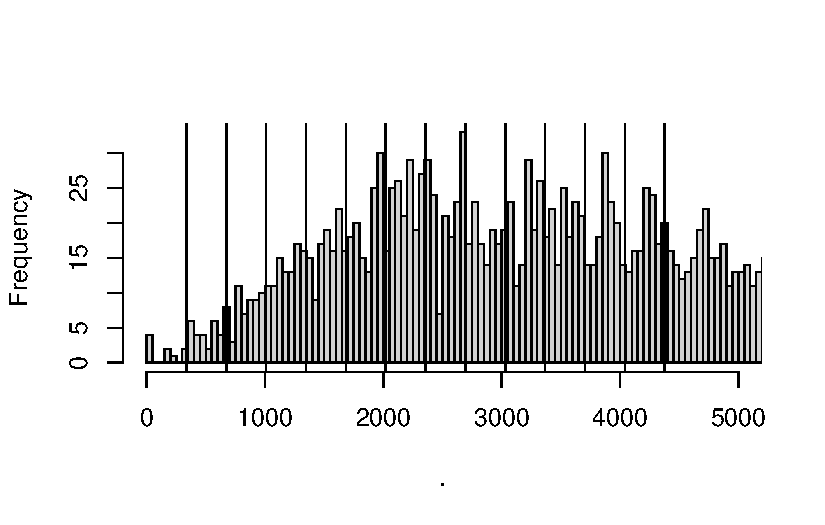
\includegraphics{Tax-Prod_files/figure-pdf/fig-revenue-hist-bunch-0-1.pdf}

}

\caption{\label{fig-revenue-hist-bunch-0}Revenue distribution Juridical
Org. 0 (81-83)}

\end{figure}

\begin{figure}

{\centering 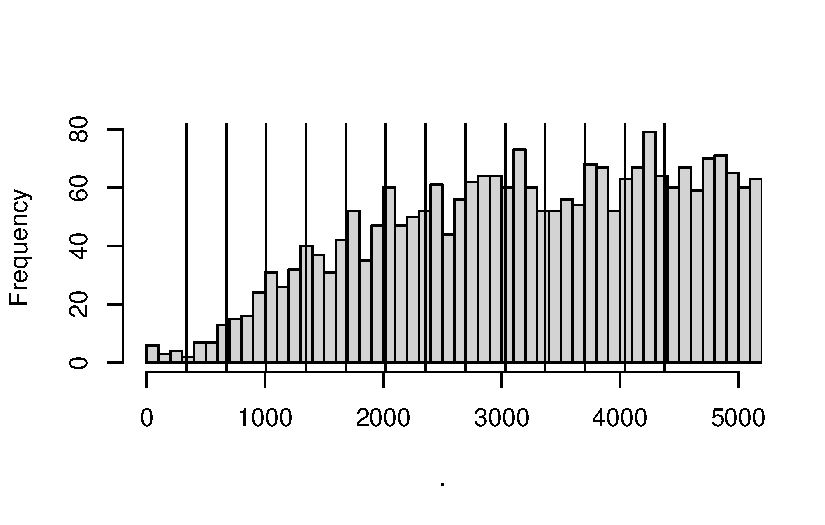
\includegraphics{Tax-Prod_files/figure-pdf/fig-revenue-hist-bunch-1-1.pdf}

}

\caption{\label{fig-revenue-hist-bunch-1}Revenue distribution Juridical
Org. 1 (81-83)}

\end{figure}

\begin{equation}\protect\hypertarget{eq-reg-tax-jo}{}{
log(s_{it})= \Phi(k_{it},l_{it},m_{it})+ \alpha_1Tax_{it}+\mathbf{\beta}_1'JurOrg_i + \beta_2'JurOrg_i\times\gamma_t+ \gamma_t + \gamma_{ind} +\gamma_{metro} + \varepsilon_{it}
}\label{eq-reg-tax-jo}\end{equation}

\hypertarget{tbl-reg-tax-jo}{}
\begin{table}
\caption{\label{tbl-reg-tax-jo}Sales tax and Juridical Organization type effect on the log share of
intermediate inputs. }\tabularnewline

\centering
\begin{tabular}[t]{l|l|l|l|l}
\hline
 & feols(log_shar..1 & feols(log_share..2 & feols(log_share..3 & feols(log_share..4\\
\hline
 & (1) & (2) & (3) & (4)\\
\hline
Dependent Var.: & \(log(s)\) & \(log(s)\) & \(log(s)\) & \(log(s)\)\\
\hline
 &  &  &  & \\
\hline
Sales Tax Rate & 0.5941** (0.1366) & 0.7719*** (0.0976) & 0.7719*** (0.0973) & 0.7520*** (0.1001)\\
\hline
J. Org. (0) & 0.4412** (0.1081) & 0.4285** (0.1088) & 0.4285** (0.1082) & 0.4249** (0.1064)\\
\hline
J. Org. (1) & 0.4492** (0.1077) & 0.4429** (0.1088) & 0.4429** (0.1082) & 0.4376** (0.1069)\\
\hline
J. Org. (2) & 0.4596** (0.1145) & 0.4434** (0.1141) & 0.4434** (0.1134) & 0.4480** (0.1116)\\
\hline
J. Org. (3) & 0.2757* (0.1145) & 0.3033* (0.1109) & 0.3033* (0.1104) & 0.3023* (0.1087)\\
\hline
J. Org. (4) & 0.4509** (0.1025) & 0.4471** (0.1035) & 0.4471** (0.1029) & 0.4431** (0.1014)\\
\hline
J. Org. (5) & 0.4619** (0.1193) & 0.4534** (0.1210) & 0.4534** (0.1204) & 0.4482** (0.1189)\\
\hline
J. Org. (6) & 0.3464** (0.0979) & 0.3397** (0.0973) & 0.3397** (0.0968) & 0.3369** (0.0964)\\
\hline
J. Org. (7) & 0.5487** (0.1571) & 0.5196** (0.1579) & 0.5196** (0.1571) & 0.5229** (0.1553)\\
\hline
J. Org. (8) & 0.2637. (0.1430) & 0.3024. (0.1377) & 0.3024. (0.1370) & 0.3068* (0.1349)\\
\hline
Fixed-Effects: & ----------------- & ------------------ & ------------------ & ------------------\\
\hline
Industry & No & Yes & Yes & Yes\\
\hline
Year & No & No & Yes & Yes\\
\hline
Metro Area & No & No & No & Yes\\
\hline
_______________ & _________________ & __________________ & __________________ & __________________\\
\hline
S.E.: Clustered & by: Industry & Year & by: Industry & Year & by: Industry & Year & by: Industry & Year\\
\hline
Observations & 41,467 & 41,467 & 41,467 & 41,467\\
\hline
R2 & 0.57951 & 0.59731 & 0.59731 & 0.60142\\
\hline
Within R2 & -- & 0.54058 & 0.53633 & 0.53876\\
\hline
\end{tabular}
\end{table}

\begin{equation}\protect\hypertarget{eq-reg-tax-fp}{}{
log(s_{it})= \Phi(k_{it},l_{it},m_{it})+ \mathbf{\beta}_1'JurOrg_i + \beta_2FiscalPd+\beta_2'JurOrg_i\times FiscalPd + \gamma_t + \gamma_{ind} +\gamma_{metro} + \varepsilon_{it}
}\label{eq-reg-tax-fp}\end{equation}

\hypertarget{tbl-reg-fiscal-p}{}
\begin{table}
\caption{\label{tbl-reg-fiscal-p}Juridical Organization type per fiscal period effect on the log share of
intermediate inputs. }\tabularnewline

\centering
\begin{tabular}[t]{l|l|l|l|l}
\hline
 & ..1 & ..2 & ..3 & ..4\\
\hline
 & (1) & (2) & (3) & (4)\\
\hline
Dependent Var.: & \(log(s)\) & \(log(s)\) & \(log(s)\) & \(log(s)\)\\
\hline
 &  &  &  & \\
\hline
J. Org. (0) x 83-86 fiscal period & -0.1112 (0.0647) & -0.1134 (0.0643) & -0.1019 (0.0612) & -0.1035 (0.0637)\\
\hline
J. Org. (1) x 83-86 fiscal period & -0.1163. (0.0619) & -0.1171. (0.0622) & -0.1091. (0.0592) & -0.1113. (0.0613)\\
\hline
J. Org. (2) x 83-86 fiscal period & -0.1462 (0.0888) & -0.1444 (0.0896) & -0.1308 (0.0866) & -0.1321 (0.0887)\\
\hline
J. Org. (3) x 83-86 fiscal period & -0.0793 (0.0605) & -0.0853 (0.0614) & -0.0779 (0.0583) & -0.0808 (0.0604)\\
\hline
J. Org. (4) x 83-86 fiscal period & -0.1401. (0.0722) & -0.1384. (0.0733) & -0.1260 (0.0699) & -0.1276 (0.0720)\\
\hline
J. Org. (5) x 83-86 fiscal period & -0.1068 (0.0592) & -0.1047 (0.0596) & -0.0963 (0.0570) & -0.0982 (0.0592)\\
\hline
J. Org. (6) x 83-86 fiscal period & -0.1566. (0.0827) & -0.1530. (0.0816) & -0.1474. (0.0805) & -0.1495. (0.0824)\\
\hline
J. Org. (7) x 83-86 fiscal period & -0.1840** (0.0545) & -0.1856** (0.0539) & -0.1747** (0.0516) & -0.1777** (0.0542)\\
\hline
J. Org. (8) x 83-86 fiscal period & -0.1989** (0.0540) & -0.1980* (0.0646) & -0.1896* (0.0612) & -0.1923* (0.0628)\\
\hline
J. Org. (0) x 87-91 fiscal period & -0.2045*** (0.0224) & -0.2146*** (0.0203) & -0.1936*** (0.0209) & -0.1938*** (0.0229)\\
\hline
J. Org. (1) x 87-91 fiscal period & -0.1942*** (0.0224) & -0.2028*** (0.0226) & -0.1858*** (0.0223) & -0.1856*** (0.0243)\\
\hline
J. Org. (2) x 87-91 fiscal period & -0.1675. (0.0832) & -0.1776. (0.0805) & -0.1536. (0.0794) & -0.1541. (0.0813)\\
\hline
J. Org. (3) x 87-91 fiscal period & -0.1631*** (0.0254) & -0.1832*** (0.0232) & -0.1676*** (0.0228) & -0.1667*** (0.0242)\\
\hline
J. Org. (4) x 87-91 fiscal period & -0.2694*** (0.0439) & -0.2738*** (0.0462) & -0.2533*** (0.0455) & -0.2533*** (0.0465)\\
\hline
J. Org. (5) x 87-91 fiscal period & -0.1904*** (0.0272) & -0.1995*** (0.0262) & -0.1803*** (0.0265) & -0.1799*** (0.0279)\\
\hline
J. Org. (6) x 87-91 fiscal period & -0.1127 (0.0655) & -0.1256. (0.0667) & -0.1120 (0.0634) & -0.1117 (0.0644)\\
\hline
J. Org. (7) x 87-91 fiscal period & -0.2389*** (0.0500) & -0.2454*** (0.0521) & -0.2212** (0.0520) & -0.2209** (0.0530)\\
\hline
J. Org. (8) x 87-91 fiscal period & -0.2547*** (0.0393) & -0.2593*** (0.0558) & -0.2429** (0.0547) & -0.2424** (0.0548)\\
\hline
Fixed-Effects: & ------------------- & ------------------- & ------------------- & -------------------\\
\hline
Industry & No & Yes & Yes & Yes\\
\hline
Metro Area & No & No & Yes & Yes\\
\hline
Year & No & No & No & Yes\\
\hline
_________________________________ & ___________________ & ___________________ & ___________________ & ___________________\\
\hline
S.E.: Clustered & by: Industry & Year & by: Industry & Year & by: Industry & Year & by: Industry & Year\\
\hline
Observations & 41,467 & 41,467 & 41,467 & 41,467\\
\hline
R2 & 0.56230 & 0.57858 & 0.58367 & 0.58420\\
\hline
Within R2 & -- & 0.51921 & 0.52254 & 0.51882\\
\hline
\end{tabular}
\end{table}

\hypertarget{references}{%
\section*{References}\label{references}}
\addcontentsline{toc}{section}{References}

\renewcommand{\bibsection}{}
\bibliography{biblio/export.bib,biblio/export2.bib,biblio/export3.bib,biblio/export31072022.bib,biblio/b100422.bib,biblio/b270123.bib}




\end{document}
